\documentclass[12pt,onecolumn]{article}
\usepackage{listings}
\usepackage{float}
\usepackage{mathtools}
\usepackage{hyperref}
\usepackage[russian]{babel}
\everymath{\displaystyle}
\usepackage{placeins}
\usepackage[table,xcdraw]{xcolor}
\usepackage{geometry}
\geometry{
  a4paper,
  top=25mm, 
  right=15mm, 
  bottom=25mm, 
  left=15mm
}

\begin{document}
\setcounter{tocdepth}{4}
\begin{center}
    Санкт-Петербургский Национальный Исследовательский\\ 
    Университет ИТМО\\
    Мегафакультет Компьютерных Технологий и Управления\\
    Факультет Программной Инженерии и Компьютерной Техники \\
    
\includegraphics[scale=0.3]{itm.jpg} % нужно закинуть картинку логтипа в папку с отчетом
\end{center}
\vspace{1cm}


\begin{center}
    \large \textbf{Вариант №255687}\\
    \textbf{Лабораторная работа №5}\\
    по дисциплине\\
    \textbf{Программирование}
\end{center}

\vspace{2cm}

\begin{flushright}
  Выполнил Студент  группы P3116\\
  \textbf{Student's name}\\
  Преподаватель: \\
  \textbf{Teacher's name}\\
\end{flushright}

\vspace{10cm}
\begin{center}
    г. Санкт-Петербург\\
    2021г.
\end{center}
\newpage
\tableofcontents
\newpage
\section{Текст задания}
Реализовать консольное приложение, которое реализует управление коллекцией объектов в интерактивном режиме. В коллекции необходимо хранить объекты класса \textcolor{red}{Route}, описание которого приведено ниже.\\
\textbf{Разработанная программа должна удовлетворять следующим требованиям:}
\begin{itemize}
    \item Класс, коллекцией экземпляров которого управляет программа, должен реализовывать сортировку по умолчанию.
    \item Все требования к полям класса (указанные в виде комментариев) должны быть выполнены.
    \item Для хранения необходимо использовать коллекцию типа \textcolor{red}{java.util.LinkedHashSet}
    \item При запуске приложения коллекция должна автоматически заполняться значениями из файла.
    \item Имя файла должно передаваться программе с помощью: \textbf{переменная окружения}.
    \item Данные должны храниться в файле в формате \textcolor{red}{csv}
    \item Чтение данных из файла необходимо реализовать с помощью класса \textcolor{red}{java.io.BufferedReader}
    \item Запись данных в файл необходимо реализовать с помощью класса \textcolor{red}{java.io.OutputStreamWriter}
    \item Все классы в программе должны быть задокументированы в формате javadoc.
    \item Программа должна корректно работать с неправильными данными (ошибки пользовательского ввода, отсутсвие прав доступа к файлу и т.п.).
\end{itemize}
\textbf{В интерактивном режиме программа должна поддерживать выполнение следующих команд:}
\begin{itemize}
    \item \textcolor{red}{help} : вывести справку по доступным командам
    \item \textcolor{red}{info} : вывести в стандартный поток вывода информацию о коллекции (тип, дата инициализации, количество элементов и т.д.)
    \item \textcolor{red}{show} : вывести в стандартный поток вывода все элементы коллекции в строковом представлении
    \item \textcolor{red}{add $\{$elemen$\}$} : добавить новый элемент в коллекцию
    \item \textcolor{red}{update id $\{$element$\}$} : обновить значение элемента коллекции, id которого равен заданному
    \item \textcolor{red}{remove$\_$by$\_$id id} : удалить элемент из коллекции по его id
    \item \textcolor{red}{clear} : очистить коллекцию
    \item \textcolor{red}{save} : сохранить коллекцию в файл
    \item \textcolor{red}{execute$\_$script file$\_$name} : считать и исполнить скрипт из указанного файла. В скрипте содержатся команды в таком же виде, в котором их вводит пользователь в интерактивном режиме
    \item \textcolor{red}{exit} : завершить программу (без сохранения в файл)
    \item \textcolor{red}{add$\_$if$\_$max $\{$element$\}$} : добавить новый элемент в коллекцию, если его значение превышает значение наибольшего элемента этой коллекции
    \item \textcolor{red}{remove$\_$lower $\{$element$\}$} : удалить из коллекции все элементы, меньшие, чем заданный
    \item \textcolor{red}{history} : вывести последние 10 команд (без их аргументов)
    \item \textcolor{red}{remove$\_$all$\_$by$\_$distance distance} : удалить из коллекции все элементы, значение поля distance которого эквивалентно заданному
    \item \textcolor{red}{min$\_$by$\_$distance} : вывести любой объект из коллекции, значение поля distance которого является минимальным
    \item \textcolor{red}{max$\_$by$\_$creation$\_$date} : вывести любой объект из коллекции, значение поля creationDate которого является максимальным
\end{itemize}
\textbf{Формат ввода команд:}
\begin{itemize}
    \item Все аргументы команды, являющиеся стандартными типами данных (примитивные типы, классы-оболочки, String, классы для хранения дат), должны вводиться в той же строке, что и имя команды.
    \item Все составные типы данных (объекты классов, хранящиеся в коллекции) должны вводиться по одному полю в строку.
    \item При вводе составных типов данных пользователю должно показываться приглашение к вводу, содержащее имя поля (например, "Введите дату рождения:")
    \item Если поле является enum'ом, то вводится имя одной из его констант (при этом список констант должен быть предварительно выведен).
    \item При некорректном пользовательском вводе (введена строка, не являющаяся именем константы в enum'е; введена строка вместо числа; введённое число не входит в указанные границы и т.п.) должно быть показано сообщение об ошибке и предложено повторить ввод поля.
    \item Для ввода значений null использовать пустую строку.
    \item Поля с комментарием "Значение этого поля должно генерироваться автоматически" не должны вводиться пользователем вручную при добавлении.
\end{itemize}
\textbf{Описание хранимых в коллекции классов:}
\begin{verbatim}
    public class Route {
    private int id; //Значение поля должно быть больше 0, Значение этого поля должно быть уникальным, Значение этого поля должно генерироваться автоматически
    private String name; //Поле не может быть null, Строка не может быть пустой
    private Coordinates coordinates; //Поле не может быть null
    private java.time.LocalDate creationDate; //Поле не может быть null, Значение этого поля должно генерироваться автоматически
    private Location from; //Поле не может быть null
    private Location to; //Поле не может быть null
    private Long distance; //Поле не может быть null, Значение поля должно быть больше 1
}
public class Coordinates {
    private Double x; //Максимальное значение поля: 669, Поле не может быть null
    private double y;
}
public class Location {
    private Integer x; //Поле не может быть null
    private float y;
    private double z;
}
public class Location {
    private Float x; //Поле не может быть null
    private Long y; //Поле не может быть null
    private String name; //Поле не может быть null
}
\end{verbatim}
\newpage
\section{Диаграмма классов объектной модели.}
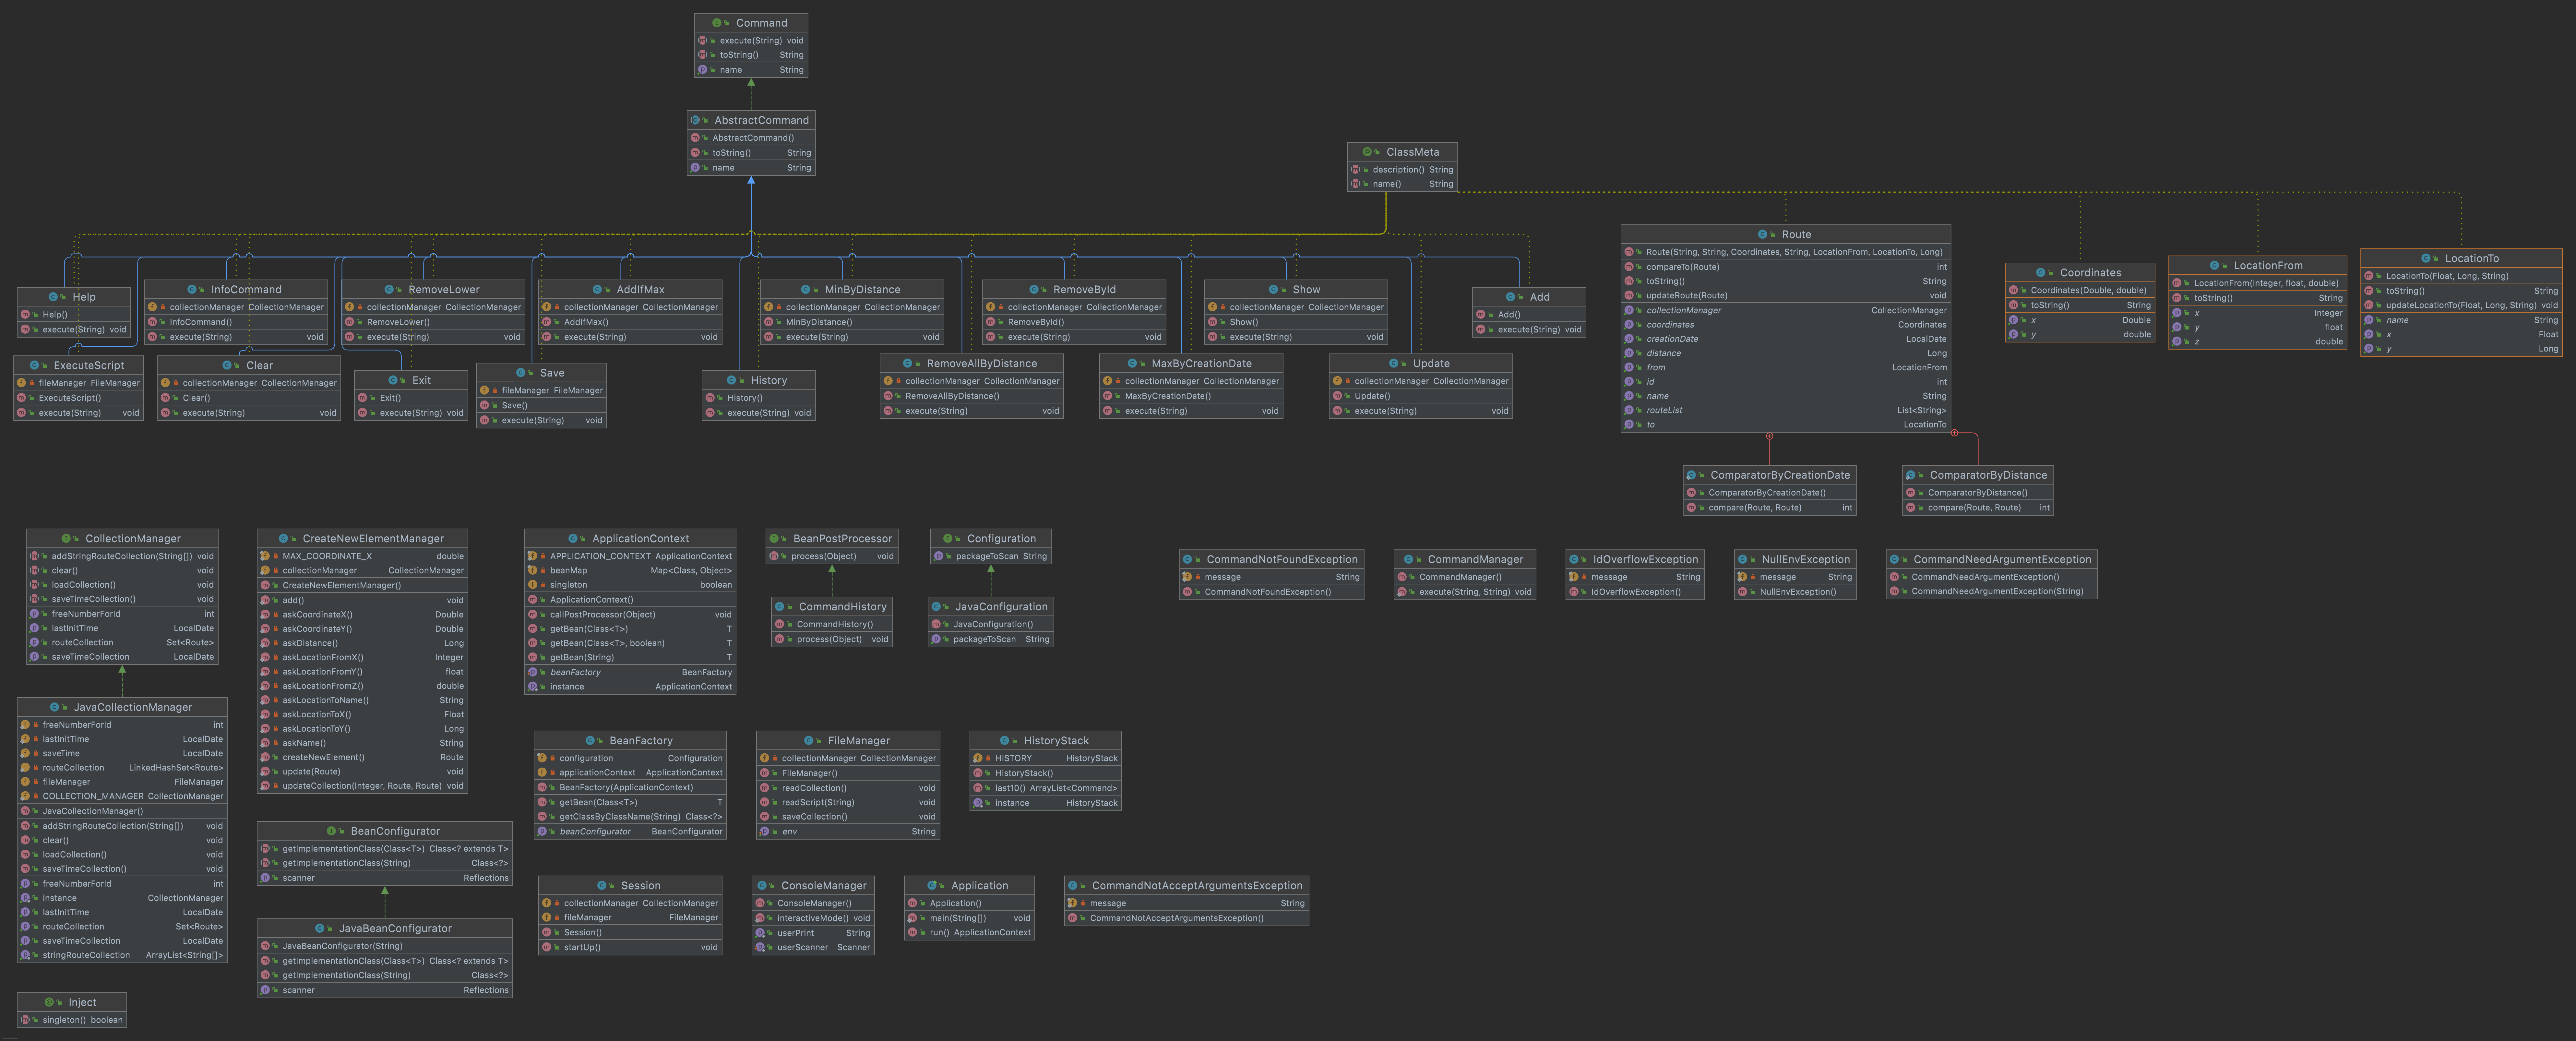
\includegraphics[scale=0.1]{UML.png}
\section{Исходный код программы}
https://github.com/AaLexUser/ProgaLab5
\section{Выводы по работе}
В этой лабораторной работе я познакомился:
\begin{itemize}
    \item с коллекциями в Java
    \item с Java i/o
\end{itemize}
\end{document}